% \pagebreak[4]
% \hspace*{1cm}
% \pagebreak[4]
% \hspace*{1cm}
% \pagebreak[4]

\chapter{Mélange d'outils}

\graphicspath{ {Chapter2/Chapter2Figs/PNG/}
  {Chapter2/Chapter2Figs/PDF/} {Chapter2/Chapter2Figs/} }

Avant de commencer, précisons juste quelques notions liées aux
déformations à base de cage:
\begin{itemize}
\item{\textit{Coordonnée :}} On définit la coordonnée d'un point comme
  étant une combinaison linéaire pondérée des positions sommets de sa
  cage.
\item{\textit{Poids :}} On appelle poids le coefficient associé à un
  sommet de la cage lors du calcul de la coordonnée d'un point de
  l'espace.\\
\end{itemize}

Chaque type d'outil (point, courbe, surface et volume) permet de
déformer l'espace de façon plus ou moins locale. Les points et courbes
sont plus adaptés aux déformations locales, c'est-à-dire ne modifiant
qu'une certaine zone de l'espace. Les surfaces et volumes sont, quant
à eux, utilisés lors de déformations plus globales, modifiant tout
l'espace contenu en leur intérieur.

Pourtant, sur le même ensemble de points, un utilisateur pourrait
souhaiter réaliser des déformations à la fois locales et globales. Les
techniques les plus utilisées ces dernières années, à savoir les
\textit{déformations à base de cage}, définissent des déformations
\textit{globales}. Une déformation est dite globale lorsque la
modification d'un des sommets de contrôle de l'outil influe sur
l'ensemble des points de l'espace, même de façon infinitésimale. Il
est donc nécessaire de calculer une coordonnée pour chaque point de
l'espace par rapport à tous les sommets de l'outil. De plus, pour
réaliser des déformations sur des zones précises, il faut que l'outil
soit composé d'un grand nombre de sommets, afin de diminuer
l'influence des sommets les plus éloignés de ces zones. On peut donc
dire qu'il existe un lien entre la précision d'une déformation et le
nombre de sommets de l'outil associé. Or plus il y a de sommets
composant l'outil, plus le temps de calcul des coordonnées est
important. Il n'est donc pas possible de réaliser des déformations sur
des zones très précises, sans avoir à calculer de coordonnées pour
tous les points de l'espace.

C'est sur cette problématique que les idées de mélange d'outils ont
été introduites. Pour simplifier la compréhension des déformations
appliquées, nous ne nous concentrons que dans le cas d'outils
déformant l'espace $\mathbb{R}^2$.

\section{Etat de l'art}

On peut citer \cite{JBPS11} comme étant les premiers à proposer une
méthode permettant de mélanger des outils de déformation de
différentes dimensions. C'est sur celui-ci que nous avons commencé à
travailler car la méthode nous semble proche de ce que nous souhaitons
réaliser. Une lecture approfondie de l'article nous fait comprendre
que le fonctionnement n'était pas celui que nous souhaitions. En
effet, s'ils semblent s'appuyer sur des outils ayant des dimensions
différentes en fonction des zones à déformer, la gestion interne
repose uniquement sur des déformations d'outils de dimension
topologique 0 (points). L'aspect "multidimensionnel" est donc
uniquement présent pour imposer des contraintes supplémentaires sur
les calculs de coordonnées. Par exemple pour des sommets reliés par
une arête les auteurs définissent que les poids évoluent de façon
linéaire le long de cette arête. De plus, cette méthode passe par une
minimisation de l'énergie laplacienne, nécessitant une discrétisation
de l'espace. Or c'est quelque chose que nous souhaitons éviter à cause
du temps de calcul requis par ces opérations.
\\

\cite{GPCP13} quant à eux, proposent une méthode permettant le mélange
d'outil de même dimension, en s'intéressant particulièrement aux cas
des déformations à base de surface, à travers les déformations à base
de cage.  Nous nous sommes intéressés à cet article de par sa récente
publication (2013), sa proximité avec \cite{Hur12}, un travail réalisé
par un étudiant en Master ISI en 2012, et de l'utilisation de cages de
déformation, le modèle semblant le plus pertinent parmi les outils de
dimension topologique 2 (surfaces). L'idée est de réaliser un
assemblage de différentes cages collées ensemble le long de leurs
arêtes et de considérer les coordonnées d'un point de l'espace, et pas
seulement par rapport à sa cage \textit{propre} (à comprendre la cage
englobant le point de l'espace) mais aussi par rapport aux cages
adjacentes à celle-ci.

Cet article propose au premier abord une formulation très simple. La
position d'un point de l'espace n'est plus simplement constituée d'une
combinaison linéaire des positions des sommets de sa cage propre, mais
résulte d'une interpolation linéaire entre les coordonnées calculées
par rapport à la cage propre et aux différentes cages
\textit{jointure}. Une cage jointure correspond à l'union des cages
incidentes à un sommet de la cage propre. L'avantage de cette méthode
est de localiser les déformations en les limitant au voisinage de la
cage incidente au sommet déplacé. Mais en contrepartie on peut avoir
jusqu'à $n$ coordonnées différentes pour un même point de l'espace, où
$n$ correspond au nombre de sommets de la cage propre. Car
possiblement il se peut que tous les sommets d'une cage soient
incidents à d'autres cages. Ce qui au final fait perdre un des
intérêts de la méthode, au moins en partie, à savoir la réduction de
la complexité en temps de calcul des coordonnées.

Par ailleurs cette formulation cache d'autres fonctions qui résultent
d'un procédé empirique, dont le cheminement n'est pas expliqué dans
l'article, ce qui rend la compréhension de l'utilité de ces fonctions
assez difficile.

\section{Cheminement de l'article}
Dans un premier temps, nous avons voulu reproduire le cheminement de
\cite{GPCP13}, pour comprendre quelles étaient les motivations
derrière la définition de chaque fonction. Nous nous sommes donc basés
sur la formulation globale décrite par l'article, qui exprime la
position d'un point de l'espace comme étant une interpolation linéaire
des coordonnées de la cage propre et de la cage jointure :

\begin{equation}
  p = \beta T(p)  + (1 - \beta) J(p),
  \label{MELgen}
\end{equation}

où $T(p)$ et $J(p)$ représentent les coordonnées du point p par
rapport à sa cage propre et à sa cage jointure respectivement, et
$\beta$ représente la distance au bord de la cage propre. Pour réduire
la complexité du nombre de coordonnées à calculer, nous avons choisi
de considérer une unique cage jointure pour chaque point de l'espace,
qui résulte de l'union de toutes les cages incidentes aux sommets de
la cage propre (autrement dit, notre cage jointure correspond à
l'union des cages jointures définies par \cite{GPCP13}). Ainsi, pour
chaque point de l'espace le nombre de coordonnées à calculer est de 2
au maximum (une pour la cage propre, et une pour l'éventuelle cage
jointure).

Le calcul de $\beta$ était proposé par l'article. Il s'agit de mesurer
la distance d'un point de l'espace par rapport à chaque arête à la
fois incidente à sa cage propre et à une autre cage. Pour éviter de
devoir calculer des distances euclidiennes, l'article propose de se
baser sur la coordonnée calculée pour chaque point $p$ par rapport aux
sommets de sa cage propre. Comme nous l'avons expliqué au début, la
coordonnée d'un point $p$ par rapport à une cage est calculée comme
étant une combinaison linéaire pondérée des positions des sommets de
cette cage. De ce fait, on peut considérer la distance de $p$ à un
sommet de la cage comme étant liée au poids qui a été associé à ce
sommet lors du calcul de la coordonnée. Et par extension, on peut
considérer la distance de $p$ à une arête comme étant liée à la somme
des poids associés aux sommets incidents de cette arête. Plus
précisément, plus on est proche d'une arête, plus la somme des poids
associés aux sommets incidents à cette arête va être proche de 1. A
l'inverse, plus on est loin d'une arête, plus la somme des poids
associés aux sommets de cette arête va être proche de 0. La distance à
une arête correspond donc au complément à 1 de la somme des poids
associés à chaque sommet des arêtes incidentes à plusieurs cages :

\begin{equation}
  d_e~ = (1 - \sum_{v \in e} \lambda_v)
\end{equation}

Où $e$ correspond à une arête, $v$ un sommet de $e$ et $\lambda_v$ le
poids associé au sommet v. L'article calcule donc $\beta$ comme étant
le produit de la distance de $p$ à chaque arête de la cage propre qui
sont aussi incidentes à d'autres cages :

\begin{equation}
  \beta = f(\prod_{e \in C} d_e)
\end{equation}

Où $f(x)$ est une fonction de lissage (Equation \ref{MELlis}),
permettant de faire varier la taille de la zone d'infuence du mélange,
tout en conservant un estompement progressif :

\begin{equation}
  f(x) = \frac{1}{2} sin(\pi(\frac{x}{h}-\frac{1}{2})) + \frac{1}{2}
  \label{MELlis}
\end{equation}
Où $h \in~ ]0,1]$ représente la zone d'influence de l'arête, ce qui
permet de délimiter la zone où le mélange de coordonnées doit être
fait (figure \ref{MELpar}). Sur la fonction en elle-même, l'influence
de $h$ correspond à une contraction de la fonction du domaine [0,1] au
domaine [0,h] (Figure \ref{MELfon}).

\begin{figure}[h]
  \begin{center}
    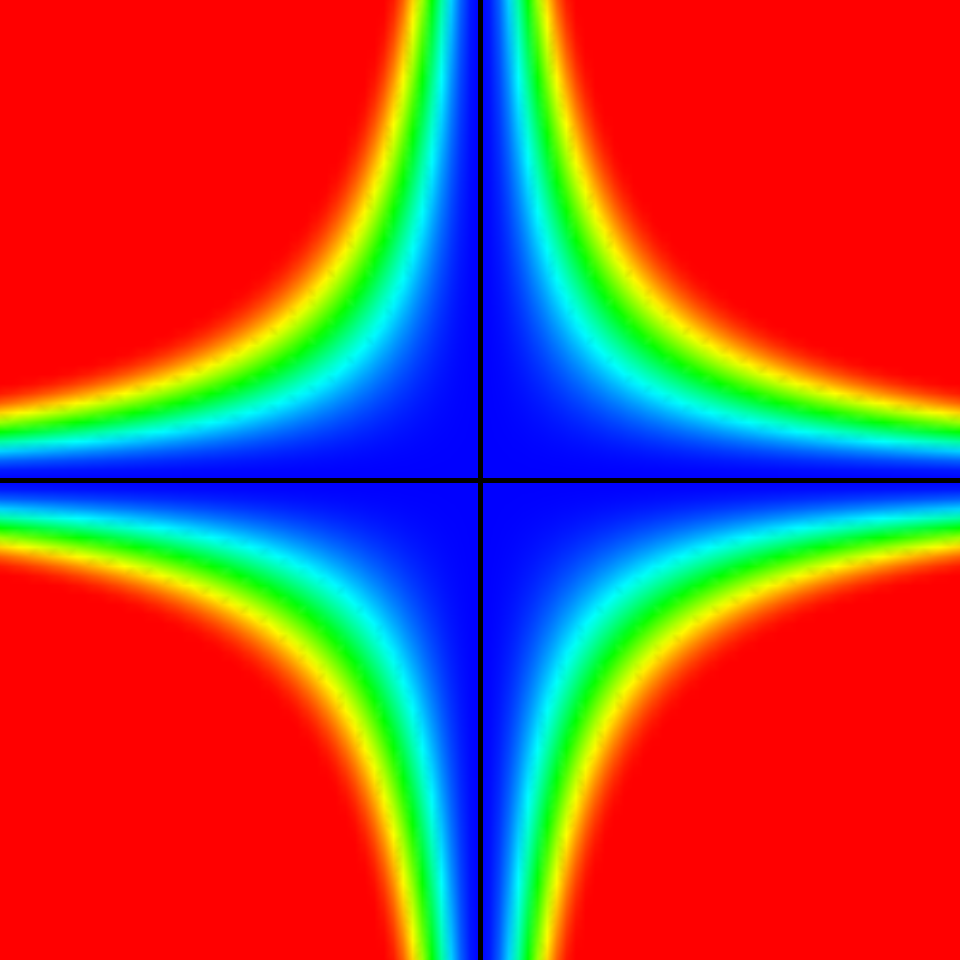
\includegraphics[scale=0.35]{starCage-0-2}
    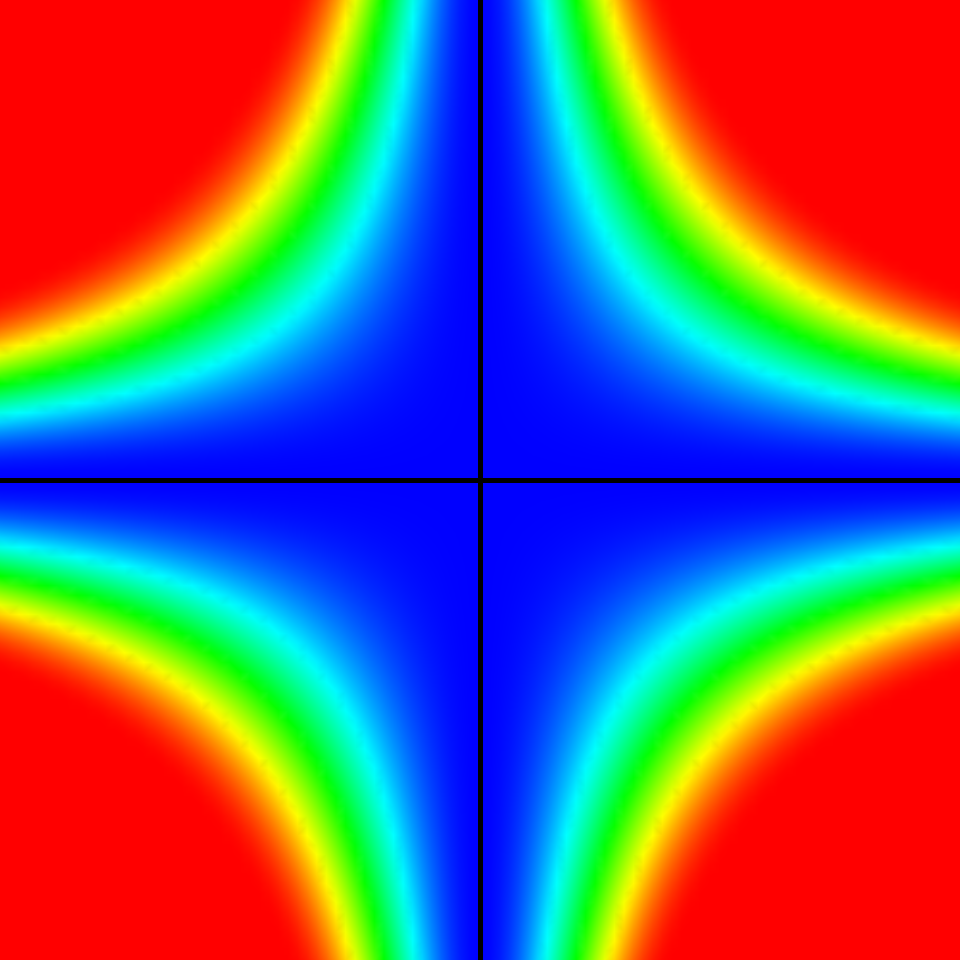
\includegraphics[scale=0.35]{starCage-0-4}
    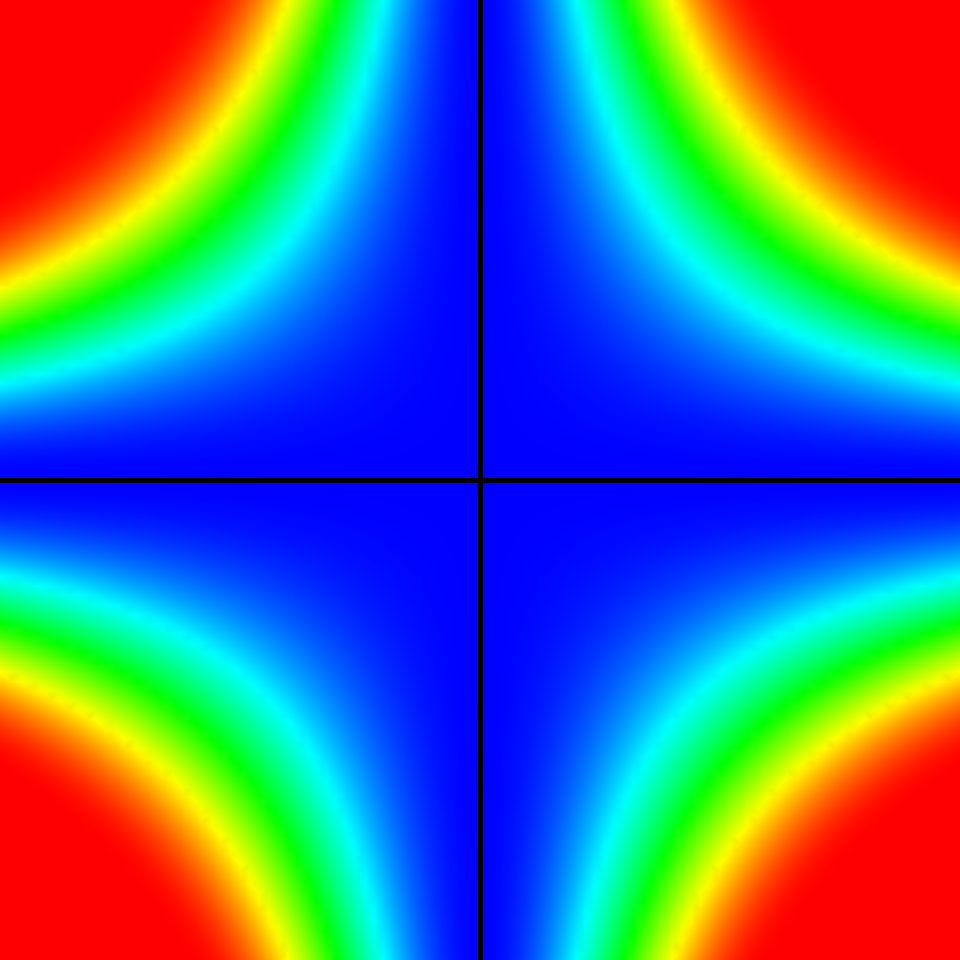
\includegraphics[scale=0.35]{starCage-0-6}
    \caption{Fonction de bordure calculée pour 4 cages (arêtes
      noires). Les variations de couleur représentent les variations
      de valeur de $\beta$ (la couleur bleu marine représentant une
      valeur de 0 et la couleur rouge une valeur de 1). En bleu les
      zones dites "de bordure" (i.e. points de l'espace proches d'une
      arête incidente à une autre cage). Valeurs de h : 0.2, 0.4 et
      0.6 pour les images à gauche, au centre et à droite
      respectivement.}
    \label{MELpar}
  \end{center}
\end{figure}

\begin{figure}[h]
  \begin{center}
    \begin{tikzpicture}
      \begin{axis}[colormap/bluered, width=0.37\textwidth,
        height=0.3\textwidth]
        \addplot gnuplot[scatter, samples=500, domain=0:0.2, mark=*,
        mark size=0.5]{1/2.*sin(pi*(x/0.2-1/2.))+1/2.};

        \addplot gnuplot[scatter, samples=500, domain=0.2:1, mark=*,
        mark size=0.5]{1};

        \draw ({axis cs:0.2,0}|-{rel axis cs:0,0}) -- ({axis
          cs:0.2,0}|-{rel axis cs:0,1}) node[near start,right] {$h =
          0.2$};
      \end{axis}
    \end{tikzpicture}
    \begin{tikzpicture}
      \begin{axis}[colormap/bluered, width=0.37\textwidth,
        height=0.3\textwidth]
        \addplot gnuplot[scatter, samples=500, domain=0:0.4, mark=*,
        mark size=0.5]{1/2.*sin(pi*(x/0.4-1/2.))+1/2.};

        \addplot gnuplot[scatter, samples=500, domain=0.4:1, mark=*,
        mark size=0.5]{1};

        \draw ({axis cs:0.4,0}|-{rel axis cs:0,0}) -- ({axis
          cs:0.4,0}|-{rel axis cs:0,1}) node[near start,right] {$h =
          0.4$};
      \end{axis}
    \end{tikzpicture}
    \begin{tikzpicture}
      \begin{axis}[colormap/bluered, width=0.37\textwidth,
        height=0.3\textwidth]
        \addplot gnuplot[scatter, samples=300, domain=0:0.6, mark=*,
        mark size=0.5]{1/2.*sin(pi*(x/0.6-1/2.))+1/2.};

        \addplot gnuplot[scatter, samples=300, domain=0.6:1, mark=*,
        mark size=0.5]{1};

        \draw ({axis cs:0.6,0}|-{rel axis cs:0,0}) -- ({axis
          cs:0.6,0}|-{rel axis cs:0,1}) node[near start,right] {$h =
          0.6$};
      \end{axis}
    \end{tikzpicture}
    \caption{Visualisation de la fonction f(x) pour différentes
      valeurs de h}
    \label{MELfon}
  \end{center}
\end{figure}

Comme $0 \leq \beta \leq 1$, on peut considérer $\beta$ comme le
pourcentage d'utilisation des coordonnées calculées par rapport à la
cage propre. D'après l'équation \ref{MELgen}, lorsque $\beta$ vaut 0
(i.e. $p$ se trouve sur une arête de la cage), la position de $p$
dépend uniquement de la coordonnée calculée par rapport à la cage
jointure $c_j$.

C'est là qu'apparaît le premier problème : Considérons une grille 2*2
constituée de 4 faces, chaque face constituant une cage. Toutes les
cages sont incidentes à un même sommet $s$. De ce fait, la zone autour
des arêtes incidentes à ce sommet est fortement influencée par la cage
jointure composée de l'union des 4 cages. Afin que la cage jointure
reste un polygone, $s$ ne doit pas être considéré comme un sommet de
la cage jointure, car il fait partie de l'intérieur de
celle-ci. L'équation \ref{MELgen} nous indique que les zones les plus
proches des arêtes ne sont influencées que par la cage jointure. Et
que, par conséquent, $s$ n'a aucune influence sur ces points. On peut
voir sur la figure \ref{MELjoi} que les points les plus proches des
arêtes incidentes à $s$ sont en bleu marine, ce qui signifie que $s$
n'a aucune influence (ou une influence très faible) sur ces points les
et une plus grande influence sur les points plus éloignés. Ce qui est
un comportement complètement contre-intuitif et la déformation
engendrée n'est pas du tout celle attendue.

\begin{figure}[h]
  \begin{center}
    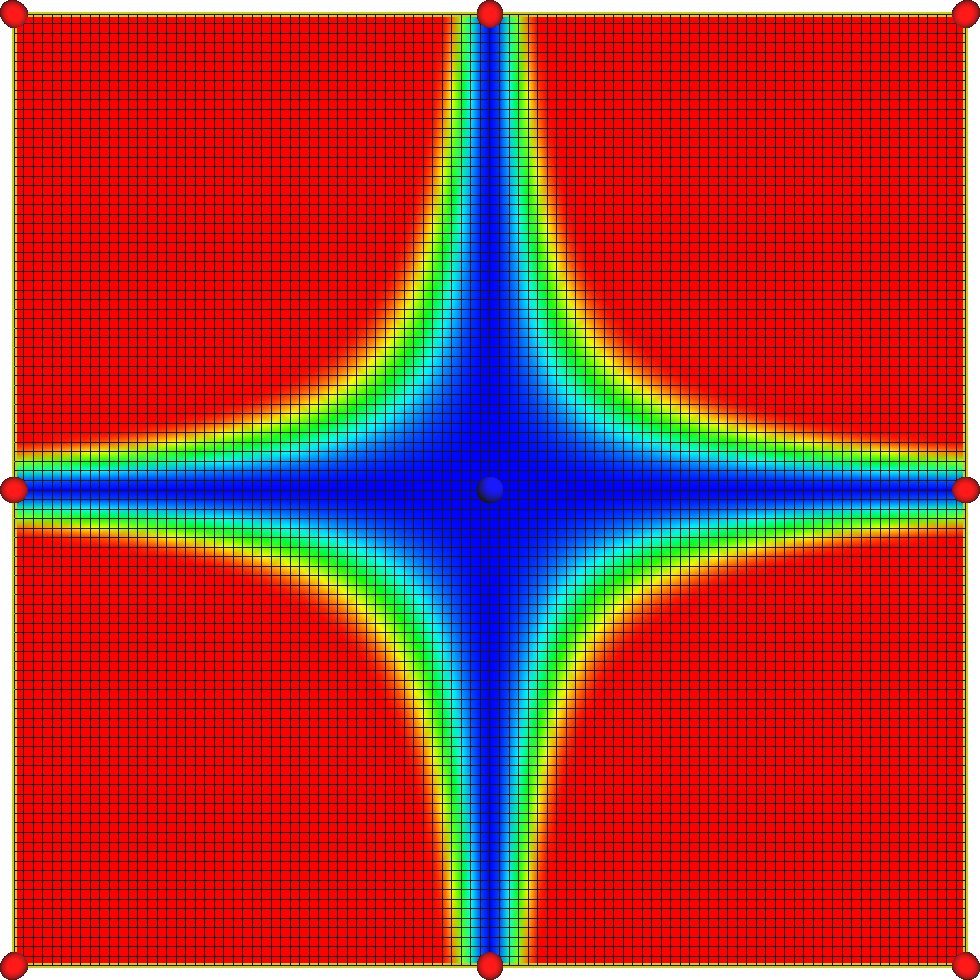
\includegraphics[scale=0.35]{starCage-jointure}
    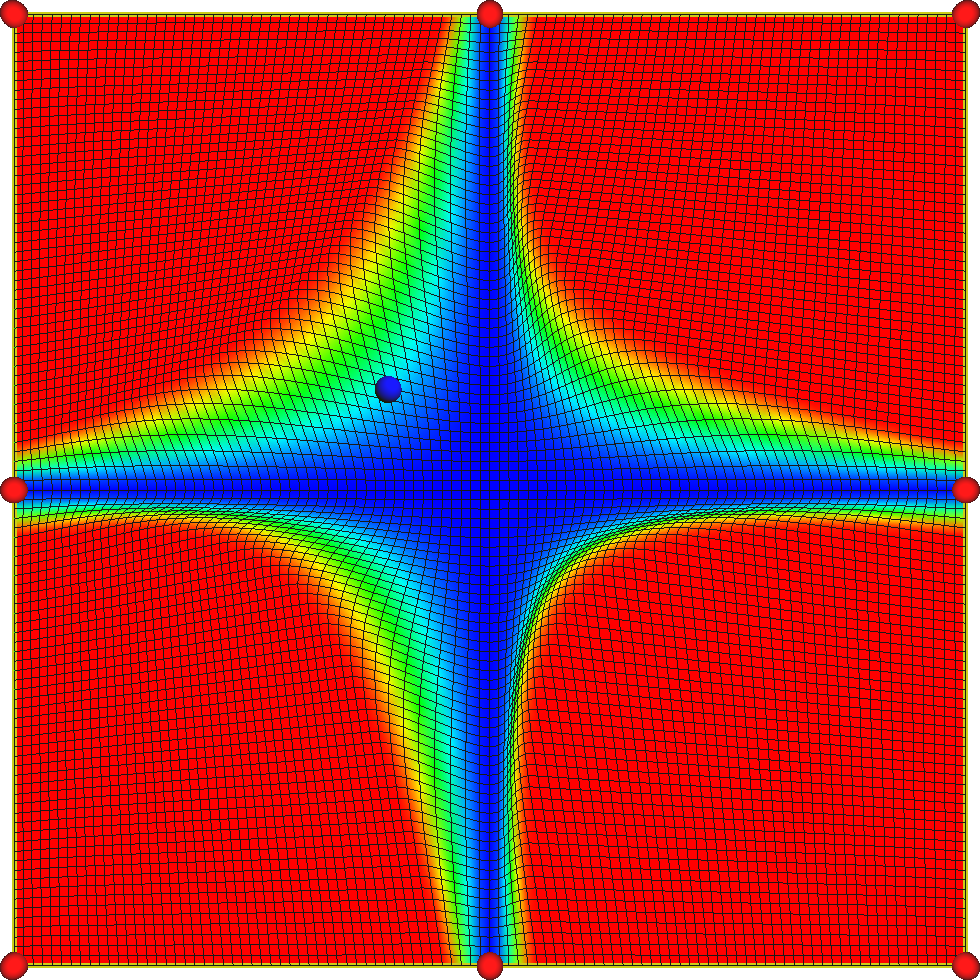
\includegraphics[scale=0.35]{starCage-jointure-deformation}
    \caption{A gauche la grille avant déformation et à droite la même
      grille après déplacement de $s$. Les boules rouges représentent
      les sommets de la cage jointure et la boule bleue représente le
      sommet $s$. Les zones en bleu ne sont pas modifiées par la
      translation de $s$.}
    \label{MELjoi}
  \end{center}
\end{figure}

De là, apparaît dans l'article la nécessité de rajouter un
comportement spécifique pour ces fameux sommets qui font partie de
l'intérieur de leur cage jointure. Ils résolvent ce problème au
travers de l'expression d'une déformation à base de points, associée
au sommet $s$. A partir de là, nous comprenons que la méthode proposée
\cite{GPCP13} n'est que le résultat d'une suite de résolutions de cas
spécifiques. Ce qui ne nous intéresse pas, car un de nos critères
principaux est l'utilisation d'une formulation simple permettant
d'exprimer les coordonnées de chaque point de façon claire. De plus,
cette méthode semble difficilement associable avec une méthode
multidimensionnelle, car elle se base sur une fusion d'outils (l'union
des cages de déformation), ce qui ne semble pas être directement
applicable pour des outils de différentes dimensions.

Nous pouvons néanmoins relever l'avancée qu'apporte cet article dans
le domaine des déformations à base de cages. En effet, grâce au
mélange de plusieurs cages, les déformations peuvent être locales,
tout en ayant un faible nombre de sommets composant les cages. De
plus, la possibilité d'utiliser conjointement plusieurs systèmes de
coordonnées différents permet de choisir le plus adapté aux
différentes déformations à effectuer.

C'est pour ça que la méthode proposée s'inspire de cet article, en
gardant l'esprit cette idée de localisation de la déformation et de
limitation du temps de calcul des coordonnées.

\section{Méthode proposée}
Dans le cadre de ce stage, nous avons eu l'idée est de considérer des
coordonnées \textit{étendues} pour chaque cage, au lieu de considérer
des unions de cages, et de réaliser un mélange de coordonnées pour les
points de l'espace qui sont sous l'influence de plusieurs cages. On se
base ici sur le fait que les coordonnées MVC sont définies non
seulement à l'intérieur, mais aussi à l'extérieur du polygone de
contrôle.

Pour vérifier la possibilité de réalisation d'une telle méthode, nous
avons commencé par travailler sur un exemple simple, une cage unique
déformant les points de l'espace à la fois à l'intérieur et à
l'extérieur grâce aux coordonnées MVC. Il s'agissait de voir le
comportement de la déformation, afin de savoir s'il était possible de
calculer des coordonnées à la fois à l'intérieur et à l'extérieur de
la cage, tout en permettant un passage lisse de l'un à l'autre. Car
dans la littérature, les coordonnées n'ont été utilisées que pour
déformer des points à l'intérieur du polygone et jusqu'à son bord.

Il se trouve que les coordonnées MVC sont $C^\infty$ partout, sauf au
niveau des sommets du polygone de contrôle, où elles ne sont que $C^0$
(Corrolaire 4.8 \cite{HF06}). De plus, à l'extérieur de la cage, on
peut constater que les coordonnées ne s'estompent pas. Ceci est dû à
la partition de l'unité, qui est une propriété des coordonnées
barycentriques généralisées. Cette propriété est induite par la
normalisation des poids associés à chaque sommet (Equation
\ref{MELnor}).

\begin{equation}
  \lambda_i(p) = \frac{w_i(p)}{\sum_{j=0}^n w_j(p)}
  \label{MELnor}
\end{equation}

Cette formule définit que la somme des poids associés à chaque sommet
de la cage, pour un point $p$ donné, doit valoir 1 (Equation
\ref{MELsum}) :

\begin{equation}
  \sum_{i=0}^n \lambda_i(p) = 1
  \label{MELsum}
\end{equation}

Pour expliquer en quoi cela pose un problème, regardons la
construction des coordonnées MVC pour un point $p$ donné. Dans un
premier temps on évalue l'influence de chaque sommet $v_i$, dont le
calcul se fait par rapport au sommet voisins $v_{i-1}$ et $v_{i+1}$ :

\begin{equation}
  w_i(p) = \frac{tan(\alpha_{i-1}(p)/2) + tan(\alpha_{i}(p)/2)}{\|v_i - p\|}
\end{equation}

où $w_i(p)$ représente le poids associé au sommet $v_i$ pour le point
$p$ et $\alpha_i(p)$ l'angle en $p$ du triangle $[p,v_i,v_{i+1}]$
(Figure \ref{MELmvc}).

\begin{figure}[h]
  \begin{center}
    \scalebox{1} % Change this value to rescale the drawing.
    {
      \begin{pspicture}(0,-3.771875)(7.3034377,3.751875)
        \psdots[dotsize=0.2](2.1,3.631875)
        \psdots[dotsize=0.2](0.1,1.731875)
        \psdots[dotsize=0.2](1.68,0.411875)
        \psdots[dotsize=0.2](2.3,-3.128125)
        \psdots[dotsize=0.2](6.68,-1.748125)
        \psdots[dotsize=0.2](6.02,3.071875)
        \psdots[dotsize=0.2](3.78,1.391875)
        \psline[linewidth=0.04cm](2.32,-3.148125)(1.68,0.431875)
        \psline[linewidth=0.04cm](2.32,-3.128125)(6.72,-1.728125)
        \psline[linewidth=0.04cm](1.66,0.431875)(0.08,1.731875)
        \psline[linewidth=0.04cm](0.08,1.711875)(2.1,3.651875)
        \psline[linewidth=0.04cm](3.78,1.371875)(2.12,3.611875)
        \psline[linewidth=0.04cm](3.8,1.391875)(6.0,3.051875)
        \psline[linewidth=0.04cm](6.68,-1.768125)(6.04,3.071875)
        \psline[linewidth=0.04cm](2.1,3.631875)(5.98,3.091875)
        \psline[linewidth=0.04cm](3.78,1.371875)(6.68,-1.748125)
        \psline[linewidth=0.04cm](2.3,-3.168125)(3.78,1.371875)
        \psline[linewidth=0.04cm](1.7,0.391875)(3.76,1.351875)
        \psline[linewidth=0.04cm](0.1,1.711875)(3.82,1.391875)
        \rput{-135.0}(5.4728017,4.9906588){\psarc[linewidth=0.04](3.77,1.361875){0.5515433}{27.758541}{174.64418}}
        \usefont{T1}{ptm}{m}{n} \rput(2.2734375,-3.493125){\large
          $v_{i-1}$} \usefont{T1}{ptm}{m}{n}
        \rput(6.6734376,-2.213125){\large $v_i$}
        \usefont{T1}{ptm}{m}{n} \rput(5.9734373,3.486875){\large
          $v_{i+1}$} \usefont{T1}{ptm}{m}{n}
        \rput(3.9634376,0.366875){\large $\alpha_{i-1}$}
        \usefont{T1}{ptm}{m}{n} \rput(4.7234373,1.346875){\large
          $\alpha_i$} \usefont{T1}{ptm}{m}{n}
        \rput(3.8434374,1.926875){\large $p$}
      \end{pspicture}
    }
    \caption{Visualisation du calcul de la coordonnée du point $p$ par
      rapport au sommet $v_i$}
    \label{MELmvc}
  \end{center}
\end{figure}

Les $w_i$ sont ensuite normalisés (Equation \ref{MELnor}), afin
d'obtenir des poids contenus dans le domaine [0,1]. Le problème est
lié à cette normalisation, car quand on éloigne un point $p$ de la
cage, si les $w_i(p)$ tendent vers 0 quand la distance $\|v_i - p\|$
tend vers l'infini, leur somme aussi tend vers 0. De ce fait, les
points extrémement éloignés de la cage seront aussi fortement
influencés par les déformations appliquées sur la cage. On voit donc
la nécessité de définir des zones d'influence autour de chaque cage,
afin de limiter leur champ d'action.

De plus,

\begin{figure}[h]
  \begin{center}
    \begin{tabular}{|l|c|c|c|}
      \hline
      Domaine & MVC & Harmoniques & Green\\
      \hline
      \textbf{Intérieur} & \textcolor{OliveGreen}{$C^\infty$} 
      & \textcolor{OliveGreen}{$C^\infty$} 
      & \textcolor{OliveGreen}{$C^\infty$} \\
      \hline
      \textbf{Bord} & \textcolor{Red}{$C^0$} 
      & \textcolor{Red}{$C^0$} 
      & \textcolor{Red}{$C^0$} \\
      \hline
      \textbf{Extérieur} & \textcolor{OliveGreen}{$C^\infty$} 
      & \textcolor{Red}{$C^0$}
      & \textcolor{OliveGreen}{$C^\infty$} \\
      \hline
    \end{tabular}
    \caption{Continuité des coordonnées (d'après \cite{GPCP13})}
    \label{SURcoo}
  \end{center}
\end{figure}

% ------------------------------------------------------------------------


%%% Local Variables: 
%%% mode: latex
%%% LaTeX-command: "latex -shell-escape"
%%% TeX-master: "../thesis"
%%% End: 
